\documentclass[11pt]{article}
\usepackage{graphicx}
\usepackage[margin=2.5cm]{geometry}
\usepackage{tikz}
\usepackage{indentfirst}
\usepackage{tabularx}
\usepackage{array}
\usepackage[portuguese]{babel}

\graphicspath{{./images/}}

\def\checkmark{\tikz\fill[scale=0.4](0,.35) -- (.25,0) -- (1,.7) -- (.25,.15) -- cycle;} 
\setlength{\parskip}{0.5em}

\begin{document}
	\begin{titlepage}
	\begin{center}
		
\includegraphics[width=0.6\textwidth]{logo-isec}
		
		\vspace*{\fill}
		
		\Huge
		\textbf{Interação Pessoa-Máquina}
		
		\huge
		Avaliação da Interface de dispositivos
		
		\vspace{0.5cm}
		\LARGE
		2020 - 2021
		
		\vspace{1.5cm}
		
		\textbf{TheForgotten\\merlin-twist}
		
		\begin{figure}[h]
			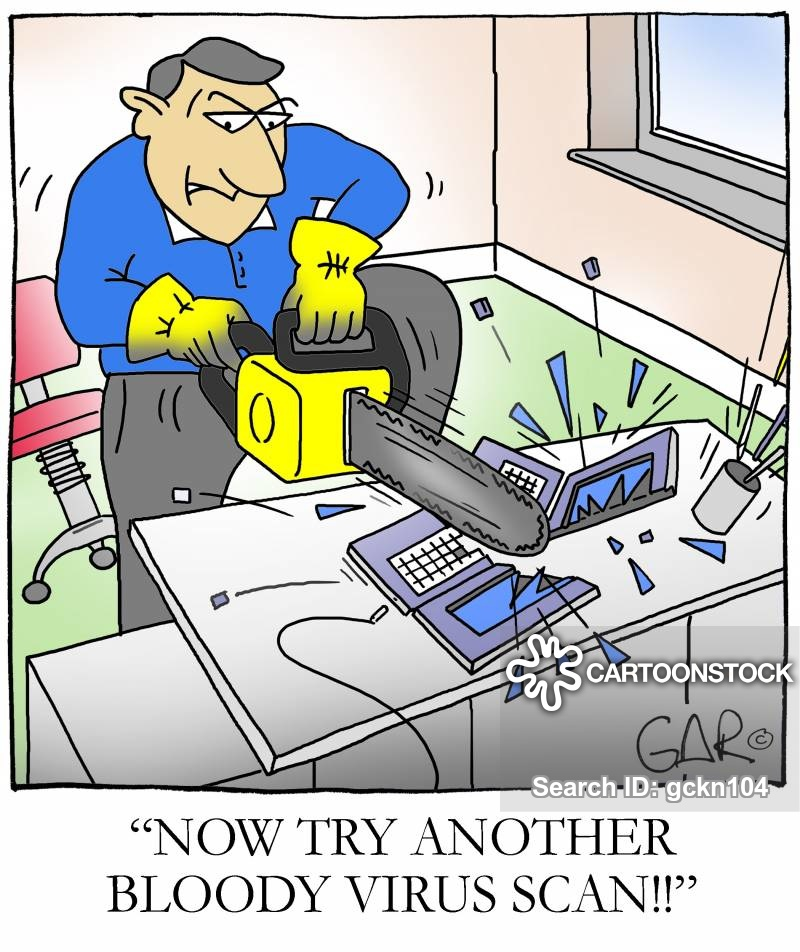
\includegraphics[width=0.5\textwidth]{boomer}
			\centering
			\caption{Homem irritado com o computador}
			\label{fig:angry-man}
		\end{figure}
		
		\vfill
		\vspace*{\fill}
		
		\normalsize
		Licenciatura de Engenharia Informática \\
		5 de março de 2021		
	\end{center}
\end{titlepage}
	
	\tableofcontents
	\pagebreak
	
	\large
	\section{Introdução}
	
	\normalsize
	\begin{center}
		\begin{tabularx}{\textwidth}{ | >{\raggedright\arraybackslash}X | }
			\hline
			\textbf{Nome do Produto:} \\ 
			store.kromgaming.com \\ \hline
			\textbf{Data do Estudo:} \\ 
			25 de abril de 2021 \\ \hline
			\textbf{Nomes dos Pesquisadores:} \\ 
			Ângelo Miguel F. Paiva \\ 
			Tomé Madail \\ \hline   
		\end{tabularx}
	\end{center}
	
	Neste trabalho, usando as \textit{10 Heurísticas de Usabilidade} (revistas) identificadas por Jakob Nielsen, será realizada a avaliação heurística de um website de aquisição de equipamento informático.
	
	\large
	\section{Relatório de Aspeto de Usabilidade}
	
	\normalsize
	\begin{center}
		\begin{tabularx}{\textwidth}{ | >{\raggedright\arraybackslash}X | >{\raggedright\arraybackslash}X | }
			\hline
			\textbf{No.} & \textbf{Problema / Bom aspeto} \\ 
			HE1 & Bom aspeto \\ \hline
			\multicolumn{2}{|l|}{\textbf{Nome:}} \\ 
			\multicolumn{2}{|l|}{O site carrega rapidamente e mostra sempre indicadores} \\ \hline
			\multicolumn{2}{|l|}{\textbf{Evidência:}} \\ 
			\multicolumn{2}{|l|}{Heurística: H2-1 Visibilidade do sistema} \\
			\multicolumn{2}{|l|}{Onde: todas as páginas} \\ 
			\multicolumn{2}{|l|}{} \\ 
			\multicolumn{2}{| >{\hsize=\dimexpr2\hsize+2\tabcolsep+\arrayrulewidth\relax}X |}{Sempre que algo necessita de algum tempo para processar, a página mostra sempre algum tipo de indicador. Para além disso, não há tempos de espera grandes.} \\ \hline  
			\multicolumn{2}{|l|}{\textbf{Explicação:}} \\ 
			\multicolumn{2}{| >{\hsize=\dimexpr2\hsize+2\tabcolsep+\arrayrulewidth\relax}X |}{A heurística referida é respeitada. O site tem sempre indicadores para tempos de espera.} \\ \hline  
			\multicolumn{2}{|l|}{\textbf{Severidade ou benefício:}} \\
			\multicolumn{2}{|l|}{\textbf{Rating:} 0 - não é um problema} \\ 
			\multicolumn{2}{|l|}{\textbf{Justificação:}} \\ 
			\multicolumn{2}{|l|}{\hspace{10mm}\textbf{Frequência:} comum} \\
			\multicolumn{2}{|l|}{\hspace{10mm}\textbf{Impacto:} fácil de superar} \\
			\multicolumn{2}{|l|}{\hspace{10mm}\textbf{Persistência:} persistente} \\
			\multicolumn{2}{| >{\hsize=\dimexpr2\hsize+2\tabcolsep+\arrayrulewidth\relax}X |}{\hspace{10mm}\textbf{Como eu medi os fatores:} o utilizador será sempre avisado por meio de indicadores sempre que a página demora um bocado a realizar o seu trabalho, apesar de raramente ter que ficar à espera.} \\ \hline  
			\multicolumn{2}{|l|}{\textbf{Possíveis soluções e/ou trade-offs:}} \\ 
			\multicolumn{2}{|l|}{-} \\ \hline  
			\multicolumn{2}{|l|}{\textbf{Relações:}} \\ 
			\multicolumn{2}{|l|}{-} \\ \hline  
		\end{tabularx}
	\end{center}
	
	\begin{center}
		\begin{tabularx}{\textwidth}{ | >{\raggedright\arraybackslash}X | >{\raggedright\arraybackslash}X | }
			\hline
			\textbf{No.} & \textbf{Problema / Bom aspeto} \\ 
			HE2 & Bom aspeto \\ \hline
			\multicolumn{2}{|l|}{\textbf{Nome:}} \\ 
			\multicolumn{2}{|l|}{O site usa a linguagem do utilizador e segue convenções} \\ \hline
			\multicolumn{2}{|l|}{\textbf{Evidência:}} \\ 
			\multicolumn{2}{|l|}{Heurística: H2-2 Correspondência entre o sistema e o mundo real} \\
			\multicolumn{2}{|l|}{Onde: todas as páginas} \\ 
			\multicolumn{2}{|l|}{} \\ 
			\multicolumn{2}{| >{\hsize=\dimexpr2\hsize+2\tabcolsep+\arrayrulewidth\relax}X |}{Toda a comunicação que a página tem com o utilizador segue convenções e usa sempre linguagem do utilizador.} \\ \hline  
			\multicolumn{2}{|l|}{\textbf{Explicação:}} \\ 
			\multicolumn{2}{| >{\hsize=\dimexpr2\hsize+2\tabcolsep+\arrayrulewidth\relax}X |}{A heurística referida é respeitada. É usada sempre linguagem que o utilizador comum entende.} \\ \hline  
			\multicolumn{2}{|l|}{\textbf{Severidade ou benefício:}} \\
			\multicolumn{2}{|l|}{\textbf{Rating:} 0 - não é um problema} \\ 
			\multicolumn{2}{|l|}{\textbf{Justificação:}} \\ 
			\multicolumn{2}{|l|}{\hspace{10mm}\textbf{Frequência:} comum} \\
			\multicolumn{2}{|l|}{\hspace{10mm}\textbf{Impacto:} fácil de superar} \\
			\multicolumn{2}{|l|}{\hspace{10mm}\textbf{Persistência:} persistente} \\
			\multicolumn{2}{| >{\hsize=\dimexpr2\hsize+2\tabcolsep+\arrayrulewidth\relax}X |}{\hspace{10mm}\textbf{Como eu medi os fatores:} o utilizador vai provavelmente entender sempre o que a página está a comunicar.} \\ \hline  
			\multicolumn{2}{|l|}{\textbf{Possíveis soluções e/ou trade-offs:}} \\ 
			\multicolumn{2}{|l|}{-} \\ \hline  
			\multicolumn{2}{|l|}{\textbf{Relações:}} \\ 
			\multicolumn{2}{|l|}{-} \\ \hline  
		\end{tabularx}
	\end{center}

	\begin{center}
		\begin{tabularx}{\textwidth}{ | >{\raggedright\arraybackslash}X | >{\raggedright\arraybackslash}X | }
			\hline
			\textbf{No.} & \textbf{Problema / Bom aspeto} \\ 
			HE3 & Bom aspeto \\ \hline
			\multicolumn{2}{|l|}{\textbf{Nome:}} \\ 
			\multicolumn{2}{|l|}{Navegação de forma livre} \\ \hline
			\multicolumn{2}{|l|}{\textbf{Evidência:}} \\ 
			\multicolumn{2}{|l|}{Heurística: H2-3 Controlo e liberdade do utilizador} \\
			\multicolumn{2}{|l|}{Onde: todas as páginas} \\ 
			\multicolumn{2}{|l|}{} \\ 
			\multicolumn{2}{| >{\hsize=\dimexpr2\hsize+2\tabcolsep+\arrayrulewidth\relax}X |}{Não obriga o utilizador a caminhos inflexíveis, sendo sempre possível voltar atrás (undo e/ou sair).} \\ \hline  
			\multicolumn{2}{|l|}{\textbf{Explicação:}} \\ 
			\multicolumn{2}{| >{\hsize=\dimexpr2\hsize+2\tabcolsep+\arrayrulewidth\relax}X |}{A heurística referida é respeitada. O utilizador consegue navegar pelo site de forma livre.} \\ \hline  
			\multicolumn{2}{|l|}{\textbf{Severidade ou benefício:}} \\
			\multicolumn{2}{|l|}{\textbf{Rating:} 0 - não é um problema} \\ 
			\multicolumn{2}{|l|}{\textbf{Justificação:}} \\ 
			\multicolumn{2}{|l|}{\hspace{10mm}\textbf{Frequência:} comum} \\
			\multicolumn{2}{|l|}{\hspace{10mm}\textbf{Impacto:} fácil de superar} \\
			\multicolumn{2}{|l|}{\hspace{10mm}\textbf{Persistência:} persistente} \\
			\multicolumn{2}{| >{\hsize=\dimexpr2\hsize+2\tabcolsep+\arrayrulewidth\relax}X |}{\hspace{10mm}\textbf{Como eu medi os fatores:} quando acontecem situações inesperadas o utilizador consegue sempre voltar atrás sem perder alterações feitas anteriormente.} \\ \hline  
			\multicolumn{2}{|l|}{\textbf{Possíveis soluções e/ou trade-offs:}} \\ 
			\multicolumn{2}{|l|}{-} \\ \hline  
			\multicolumn{2}{|l|}{\textbf{Relações:}} \\ 
			\multicolumn{2}{|l|}{-} \\ \hline  
		\end{tabularx}
	\end{center}
	
	\begin{center}
		\begin{tabularx}{\textwidth}{ | >{\raggedright\arraybackslash}X | >{\raggedright\arraybackslash}X | }
			\hline
			\textbf{No.} & \textbf{Problema / Bom aspeto} \\ 
			HE4 & Problema \\ \hline
			\multicolumn{2}{|l|}{\textbf{Nome:}} \\ 
			\multicolumn{2}{|l|}{O site é inconsistente no idioma que usa} \\ \hline
			\multicolumn{2}{|l|}{\textbf{Evidência:}} \\ 
			\multicolumn{2}{|l|}{Heurística: H2-4 Consistência e aderência a normas} \\
			\multicolumn{2}{|l|}{Onde: página "Shipping Policies", “Privacy”, “Warranty”, banners de publicidade, entre outros} \\ 
			\multicolumn{2}{|l|}{} \\ 
			\multicolumn{2}{| >{\hsize=\dimexpr2\hsize+2\tabcolsep+\arrayrulewidth\relax}X |}{Apesar de estar a navegar na página em inglês, os termos e condições estão em espanhol, bem como os banners animados a falar dos produtos.} \\ 
			\multicolumn{2}{| >{\hsize=\dimexpr2\hsize+2\tabcolsep+\arrayrulewidth\relax}X |}{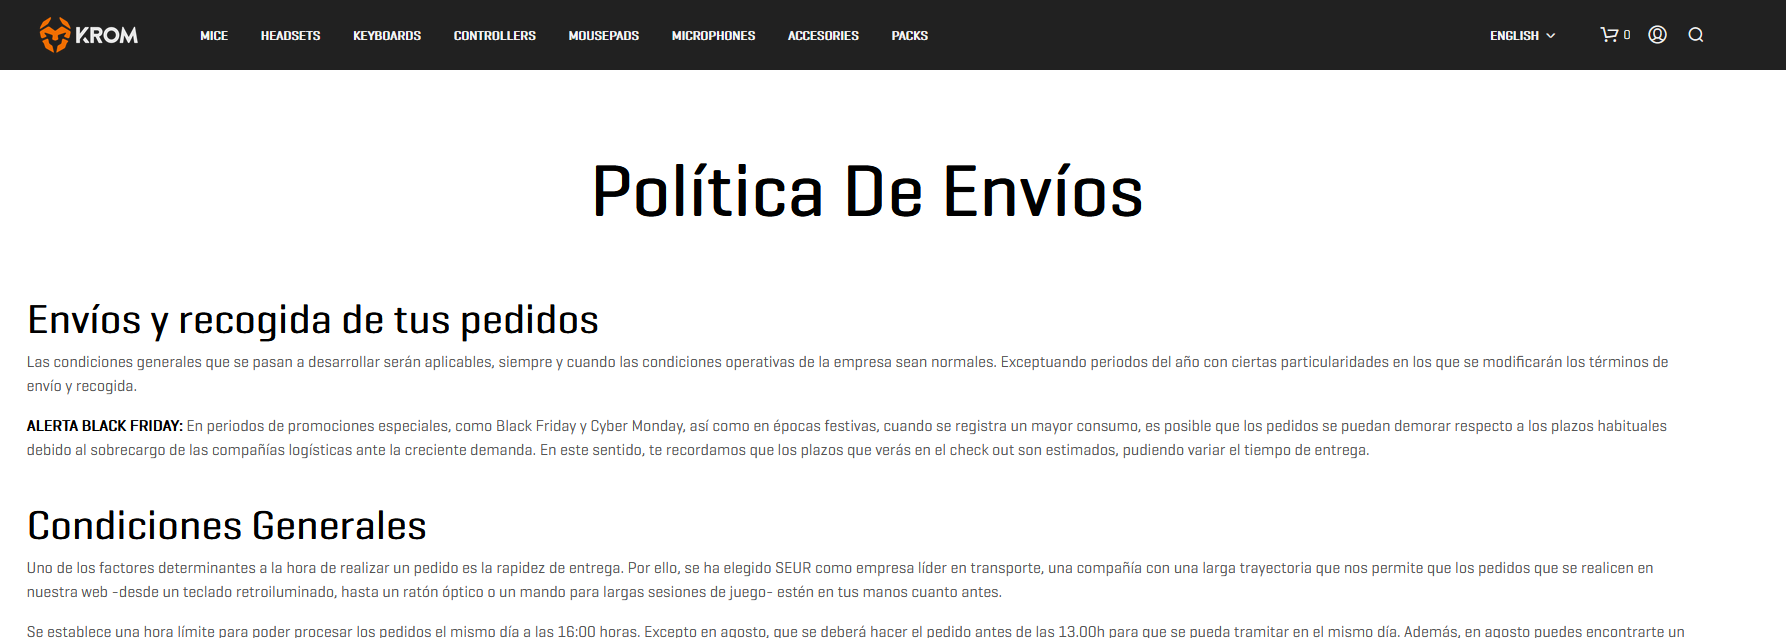
\includegraphics[width=0.9\columnwidth]{politicadeenvios-krom}} \\ \hline
			\multicolumn{2}{|l|}{\textbf{Explicação:}} \\ 
			\multicolumn{2}{| >{\hsize=\dimexpr2\hsize+2\tabcolsep+\arrayrulewidth\relax}X |}{A heurística referida não é respeitada. O site não respeita a linguagem escolhida.} \\ \hline  
			\multicolumn{2}{|l|}{\textbf{Severidade ou benefício:}} \\
			\multicolumn{2}{|l|}{\textbf{Rating:} 4 - catástrofe de usabilidade} \\ 
			\multicolumn{2}{|l|}{\textbf{Justificação:}} \\ 
			\multicolumn{2}{|l|}{\hspace{10mm}\textbf{Frequência:} comum} \\
			\multicolumn{2}{|l|}{\hspace{10mm}\textbf{Impacto:} difícil de superar} \\
			\multicolumn{2}{|l|}{\hspace{10mm}\textbf{Persistência:} persistente} \\
			\multicolumn{2}{| >{\hsize=\dimexpr2\hsize+2\tabcolsep+\arrayrulewidth\relax}X |}{\hspace{10mm}\textbf{Como eu medi os fatores:} o utilizador vai encontrar esta situação em várias páginas do site, tornando a sua navegação desconfortável se este não souber falar espanhol, e mesmo que este saiba falar espanhol, se efetivamente escolheu outro idioma não deveria ser forçado a lidar com este.} \\ \hline  
			\multicolumn{2}{|l|}{\textbf{Possíveis soluções e/ou trade-offs:}} \\ 
			\multicolumn{2}{|l|}{Traduzir as páginas e os banners para as várias linguagens que o site suporta.} \\ \hline  
			\multicolumn{2}{|l|}{\textbf{Relações:}} \\ 
			\multicolumn{2}{|l|}{-} \\ \hline  
		\end{tabularx}
	\end{center}

	\begin{center}
		\begin{tabularx}{\textwidth}{ | >{\raggedright\arraybackslash}X | >{\raggedright\arraybackslash}X | }
			\hline
			\textbf{No.} & \textbf{Problema / Bom aspeto} \\ 
			HE5 & Problema \\ \hline
			\multicolumn{2}{|l|}{\textbf{Nome:}} \\ 
			\multicolumn{2}{| >{\hsize=\dimexpr2\hsize+2\tabcolsep+\arrayrulewidth\relax}X |}{O site não questiona o utilizador mesmo que este insira um número catastrófico de produtos no carrinho} \\ \hline
			\multicolumn{2}{|l|}{\textbf{Evidência:}} \\ 
			\multicolumn{2}{|l|}{Heurística: H2-5 Prevenção de Erros} \\
			\multicolumn{2}{|l|}{Onde: carrinho de compras} \\ 
			\multicolumn{2}{|l|}{} \\ 
			\multicolumn{2}{| >{\hsize=\dimexpr2\hsize+2\tabcolsep+\arrayrulewidth\relax}X |}{O site não questiona o utilizador mesmo que este encha o carrinho com um número absurdo de produtos e com uma encomenda na casa dos milhares. (apesar de haver limitação no número máximo que o carrinho pode ter de cada produto, este varia de produto para produto de maneira inconsistente, o que me faz acreditar que este número máximo e baseado no stock que a loja tem de momento e não uma medida de segurança)} \\ 
			\multicolumn{2}{| >{\hsize=\dimexpr2\hsize+2\tabcolsep+\arrayrulewidth\relax}X |}{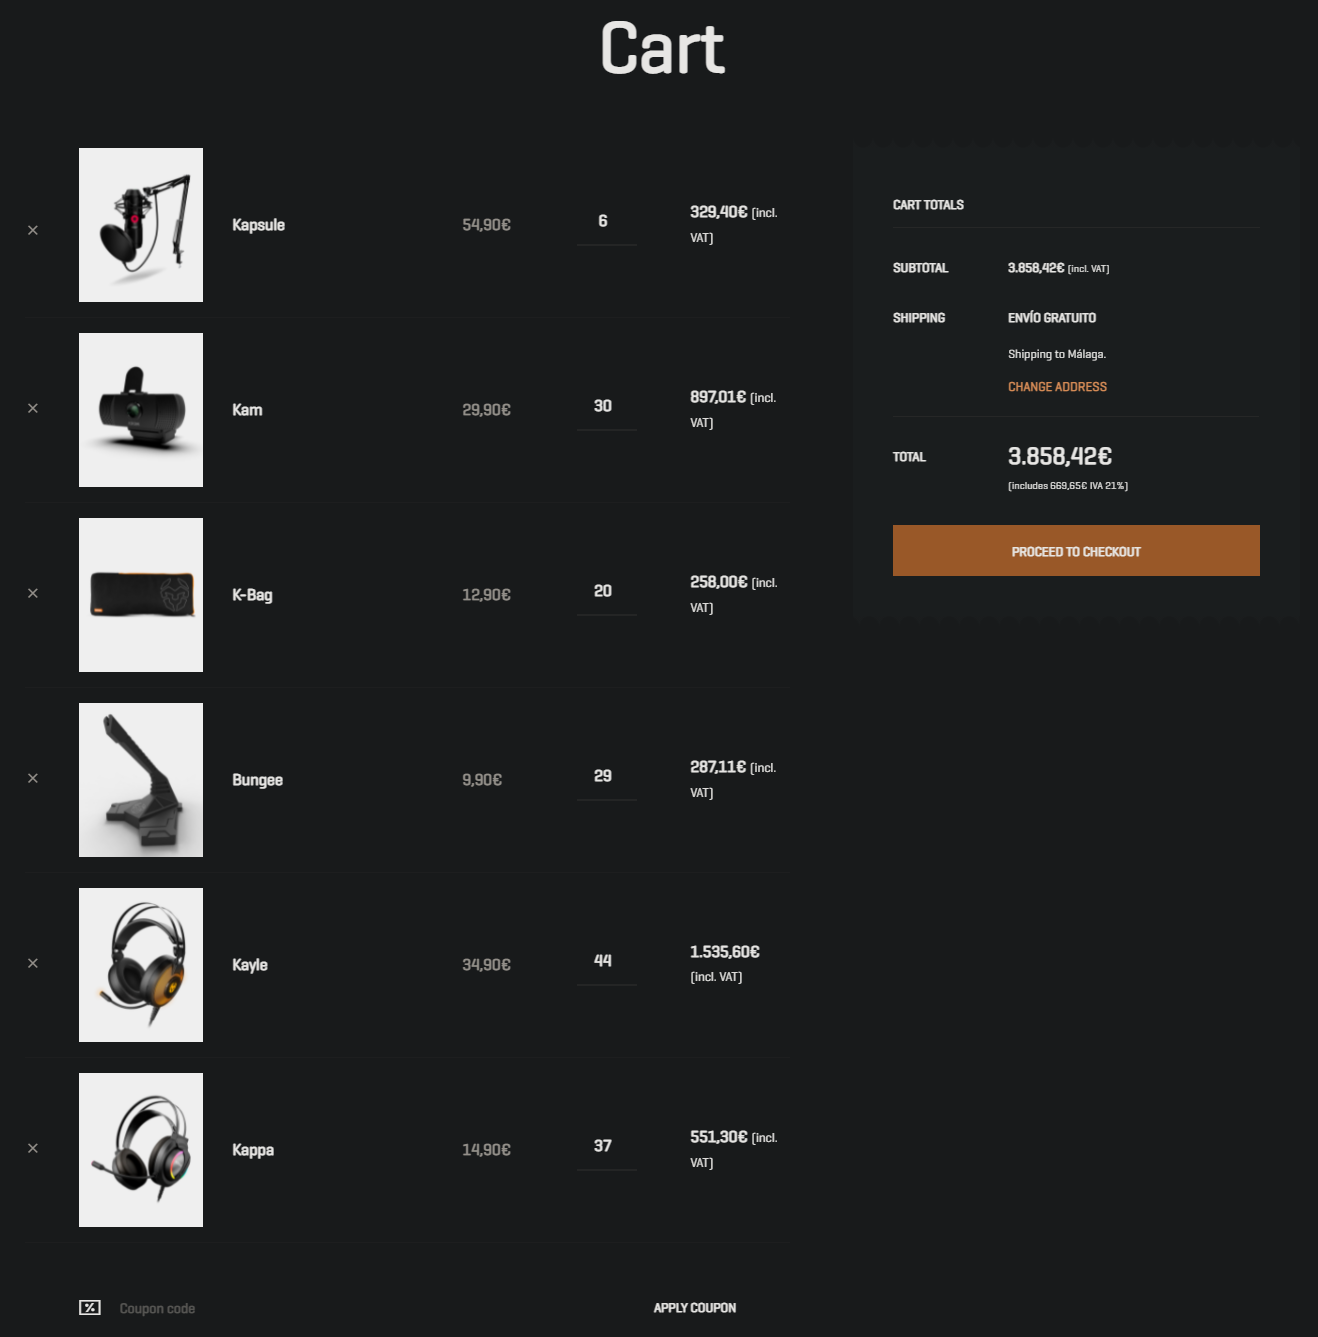
\includegraphics[width=0.5\columnwidth]{cart-krom}} \\ \hline
			\multicolumn{2}{|l|}{\textbf{Explicação:}} \\ 
			\multicolumn{2}{| >{\hsize=\dimexpr2\hsize+2\tabcolsep+\arrayrulewidth\relax}X |}{A heurística referida não é respeitada. O site não se preocupa com a quantidade de produtos nem o valor do carrinho.} \\ \hline  
			\multicolumn{2}{|l|}{\textbf{Severidade ou benefício:}} \\
			\multicolumn{2}{|l|}{\textbf{Rating:} 2 - problema de usabilidade menor} \\ 
			\multicolumn{2}{|l|}{\textbf{Justificação:}} \\ 
			\multicolumn{2}{|l|}{\hspace{10mm}\textbf{Frequência:} rara} \\
			\multicolumn{2}{|l|}{\hspace{10mm}\textbf{Impacto:} fácil de superar} \\
			\multicolumn{2}{|l|}{\hspace{10mm}\textbf{Persistência:} persistente} \\
			\multicolumn{2}{| >{\hsize=\dimexpr2\hsize+2\tabcolsep+\arrayrulewidth\relax}X |}{\hspace{10mm}\textbf{Como eu medi os fatores:} o utilizador dificilmente vai encontrar-se numa situação onde encomende um carrinho de valor tão alto tendo em conta que o site o obriga a ver o carrinho, a confirmar o mesmo, e durante o pagamento o site de terceiros também vai referir este valor.} \\ \hline  
			\multicolumn{2}{|l|}{\textbf{Possíveis soluções e/ou trade-offs:}} \\ 
			\multicolumn{2}{| >{\hsize=\dimexpr2\hsize+2\tabcolsep+\arrayrulewidth\relax}X |}{Questionar o utilizador sobre o seu carrinho a partir dum certo valor (por exemplo, e por se tratar duma loja de acessórios, 150€).} \\ \hline  
			\multicolumn{2}{|l|}{\textbf{Relações:}} \\ 
			\multicolumn{2}{|l|}{-} \\ \hline  
		\end{tabularx}
	\end{center}
		
	\begin{center}
		\begin{tabularx}{\textwidth}{ | >{\raggedright\arraybackslash}X | >{\raggedright\arraybackslash}X | }
			\hline
			\textbf{No.} & \textbf{Problema / Bom aspeto} \\ 
			HE6 & Bom aspeto \\ \hline
			\multicolumn{2}{|l|}{\textbf{Nome:}} \\ 
			\multicolumn{2}{| >{\hsize=\dimexpr2\hsize+2\tabcolsep+\arrayrulewidth\relax}X |}{Os produtos de venda são fáceis de identificar} \\ \hline
			\multicolumn{2}{|l|}{\textbf{Evidência:}} \\ 
			\multicolumn{2}{|l|}{Heurística: H2-6 Reconhecer em vez de lembrar} \\
			\multicolumn{2}{|l|}{Onde: todas as páginas} \\ 
			\multicolumn{2}{|l|}{} \\ 
			\multicolumn{2}{| >{\hsize=\dimexpr2\hsize+2\tabcolsep+\arrayrulewidth\relax}X |}{Todas as páginas de produtos possuem informação do produto, acompanhada de uma imagem, nome e preço do produto. Ainda diz se existe stock ou não.} \\ 
			\multicolumn{2}{| >{\hsize=\dimexpr2\hsize+2\tabcolsep+\arrayrulewidth\relax}X |}{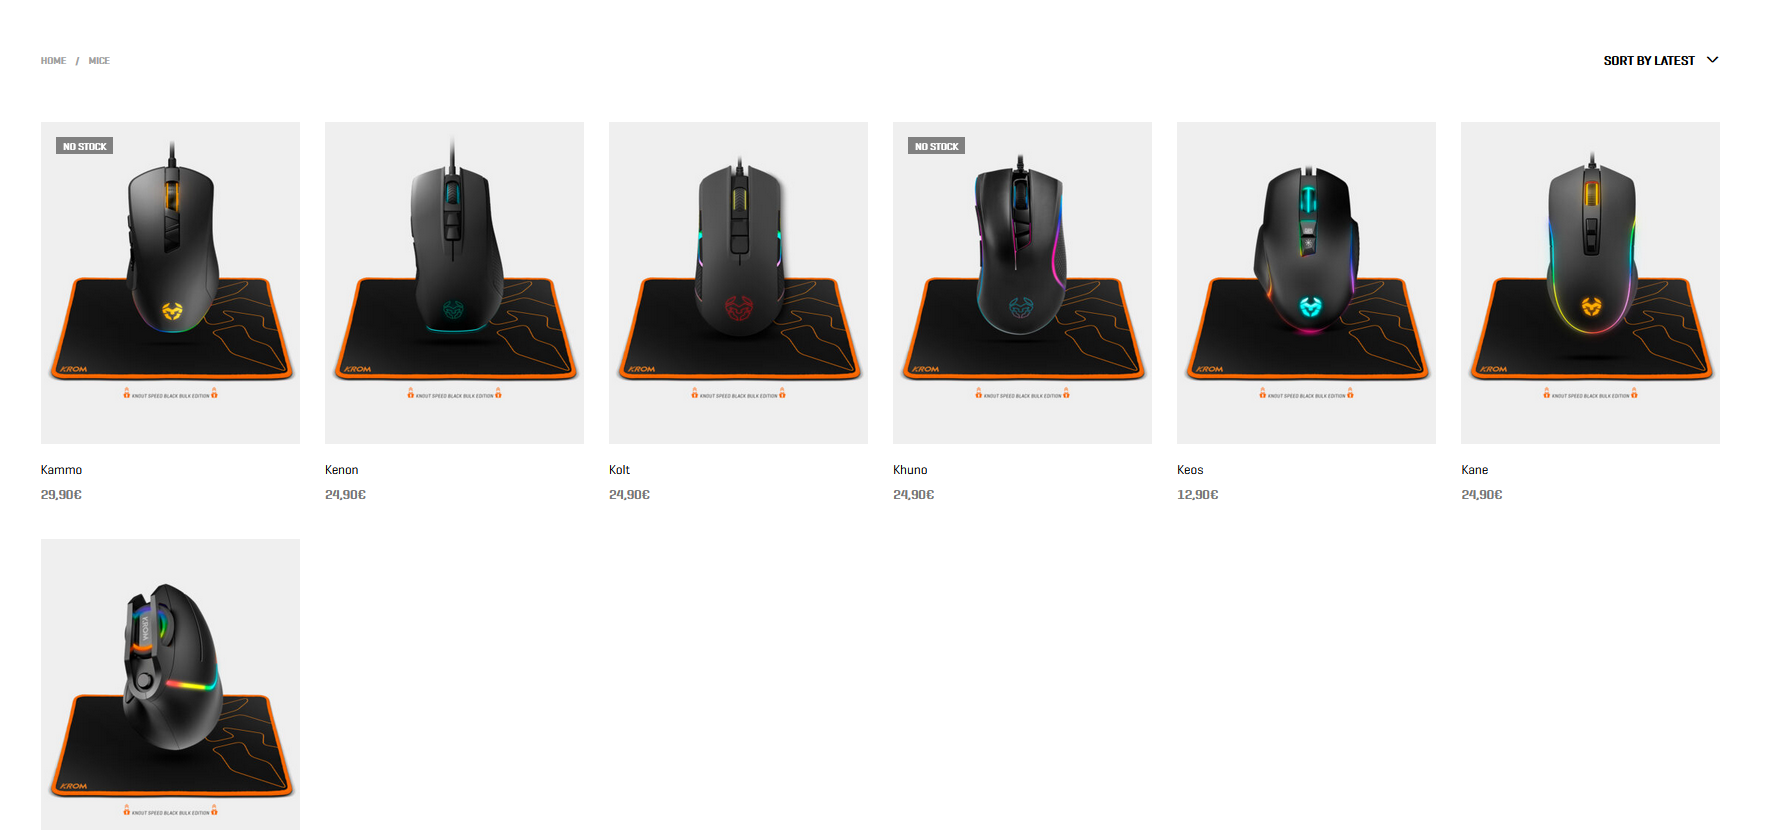
\includegraphics[width=0.9\columnwidth]{mice-krom}} \\ \hline
			\multicolumn{2}{|l|}{\textbf{Explicação:}} \\ 
			\multicolumn{2}{| >{\hsize=\dimexpr2\hsize+2\tabcolsep+\arrayrulewidth\relax}X |}{A heurística referida é respeitada. O site possui ícones com significado e as ações estão bem identificadas.} \\ \hline  
			\multicolumn{2}{|l|}{\textbf{Severidade ou benefício:}} \\
			\multicolumn{2}{|l|}{\textbf{Rating:} 0 - não é um problema} \\ 
			\multicolumn{2}{|l|}{\textbf{Justificação:}} \\ 
			\multicolumn{2}{|l|}{\hspace{10mm}\textbf{Frequência:} comum} \\
			\multicolumn{2}{|l|}{\hspace{10mm}\textbf{Impacto:} fácil de superar} \\
			\multicolumn{2}{|l|}{\hspace{10mm}\textbf{Persistência:} persistente} \\
			\multicolumn{2}{| >{\hsize=\dimexpr2\hsize+2\tabcolsep+\arrayrulewidth\relax}X |}{\hspace{10mm}\textbf{Como eu medi os fatores:} o utilizador entende sempre o que significa cada imagem e até onde o pode levar.} \\ \hline  
			\multicolumn{2}{|l|}{\textbf{Possíveis soluções e/ou trade-offs:}} \\ 
			\multicolumn{2}{| >{\hsize=\dimexpr2\hsize+2\tabcolsep+\arrayrulewidth\relax}X |}{-} \\ \hline  
			\multicolumn{2}{|l|}{\textbf{Relações:}} \\ 
			\multicolumn{2}{|l|}{-} \\ \hline  
		\end{tabularx}
	\end{center}

	\begin{center}
		\begin{tabularx}{\textwidth}{ | >{\raggedright\arraybackslash}X | >{\raggedright\arraybackslash}X | }
			\hline
			\textbf{No.} & \textbf{Problema / Bom aspeto} \\ 
			HE7 & Bom aspeto \\ \hline
			\multicolumn{2}{|l|}{\textbf{Nome:}} \\ 
			\multicolumn{2}{| >{\hsize=\dimexpr2\hsize+2\tabcolsep+\arrayrulewidth\relax}X |}{O cabeçalho do website possuí bons atalhos} \\ \hline
			\multicolumn{2}{|l|}{\textbf{Evidência:}} \\ 
			\multicolumn{2}{|l|}{Heurística: H2-7 Flexibilidade e Eficiência na utilização} \\
			\multicolumn{2}{|l|}{Onde: todas as páginas} \\ 
			\multicolumn{2}{|l|}{} \\ 
			\multicolumn{2}{| >{\hsize=\dimexpr2\hsize+2\tabcolsep+\arrayrulewidth\relax}X |}{A barra do cabecalho tem atalhos para as categorias, a homepage, para o login, o carrinho e a barra de pesquisa.} \\ 
			\multicolumn{2}{| >{\hsize=\dimexpr2\hsize+2\tabcolsep+\arrayrulewidth\relax}X |}{
\includegraphics[width=0.9\columnwidth]{bar-krom}} \\ \hline
			\multicolumn{2}{|l|}{\textbf{Explicação:}} \\ 
			\multicolumn{2}{| >{\hsize=\dimexpr2\hsize+2\tabcolsep+\arrayrulewidth\relax}X |}{A heurística referida é respeitada. O site tem uma boa barra de cabeçalho pois esta tem botões para as ações mais frequentes.} \\ \hline  
			\multicolumn{2}{|l|}{\textbf{Severidade ou benefício:}} \\
			\multicolumn{2}{|l|}{\textbf{Rating:} 0 - não é um problema} \\ 
			\multicolumn{2}{|l|}{\textbf{Justificação:}} \\ 
			\multicolumn{2}{|l|}{\hspace{10mm}\textbf{Frequência:} comum} \\
			\multicolumn{2}{|l|}{\hspace{10mm}\textbf{Impacto:} fácil de superar} \\
			\multicolumn{2}{|l|}{\hspace{10mm}\textbf{Persistência:} persistente} \\
			\multicolumn{2}{| >{\hsize=\dimexpr2\hsize+2\tabcolsep+\arrayrulewidth\relax}X |}{\hspace{10mm}\textbf{Como eu medi os fatores:} o utilizador consegue navegar o site mais eficientemente graças à boa escolha de atalhos.} \\ \hline  
			\multicolumn{2}{|l|}{\textbf{Possíveis soluções e/ou trade-offs:}} \\ 
			\multicolumn{2}{| >{\hsize=\dimexpr2\hsize+2\tabcolsep+\arrayrulewidth\relax}X |}{-} \\ \hline  
			\multicolumn{2}{|l|}{\textbf{Relações:}} \\ 
			\multicolumn{2}{|l|}{-} \\ \hline  
		\end{tabularx}
	\end{center}

	\begin{center}
		\begin{tabularx}{\textwidth}{ | >{\raggedright\arraybackslash}X | >{\raggedright\arraybackslash}X | }
			\hline
			\textbf{No.} & \textbf{Problema / Bom aspeto} \\ 
			HE8 & Bom aspeto \\ \hline
			\multicolumn{2}{|l|}{\textbf{Nome:}} \\ 
			\multicolumn{2}{| >{\hsize=\dimexpr2\hsize+2\tabcolsep+\arrayrulewidth\relax}X |}{O site possui design apelante e minimalista} \\ \hline
			\multicolumn{2}{|l|}{\textbf{Evidência:}} \\ 
			\multicolumn{2}{|l|}{Heurística: H2-8 Desenho estético e minimalista} \\
			\multicolumn{2}{|l|}{Onde: todas as páginas} \\ 
			\multicolumn{2}{|l|}{} \\ 
			\multicolumn{2}{| >{\hsize=\dimexpr2\hsize+2\tabcolsep+\arrayrulewidth\relax}X |}{O site usa uma palete de cores simples mas eficiente. Não possui botões a mais a atrapalhar a utilização do site.} \\ \hline
			\multicolumn{2}{|l|}{\textbf{Explicação:}} \\ 
			\multicolumn{2}{| >{\hsize=\dimexpr2\hsize+2\tabcolsep+\arrayrulewidth\relax}X |}{A heurística referida é respeitada. O site é apelante esteticamente.} \\ \hline  
			\multicolumn{2}{|l|}{\textbf{Severidade ou benefício:}} \\
			\multicolumn{2}{|l|}{\textbf{Rating:} 0 - não é um problema} \\ 
			\multicolumn{2}{|l|}{\textbf{Justificação:}} \\ 
			\multicolumn{2}{|l|}{\hspace{10mm}\textbf{Frequência:} comum} \\
			\multicolumn{2}{|l|}{\hspace{10mm}\textbf{Impacto:} fácil de superar} \\
			\multicolumn{2}{|l|}{\hspace{10mm}\textbf{Persistência:} persistente} \\
			\multicolumn{2}{| >{\hsize=\dimexpr2\hsize+2\tabcolsep+\arrayrulewidth\relax}X |}{\hspace{10mm}\textbf{Como eu medi os fatores:} o utilizador vai sentir-se agradado pelo aspeto do site.} \\ \hline  
			\multicolumn{2}{|l|}{\textbf{Possíveis soluções e/ou trade-offs:}} \\ 
			\multicolumn{2}{| >{\hsize=\dimexpr2\hsize+2\tabcolsep+\arrayrulewidth\relax}X |}{-} \\ \hline  
			\multicolumn{2}{|l|}{\textbf{Relações:}} \\ 
			\multicolumn{2}{|l|}{-} \\ \hline  
		\end{tabularx}
	\end{center}

	\begin{center}
		\begin{tabularx}{\textwidth}{ | >{\raggedright\arraybackslash}X | >{\raggedright\arraybackslash}X | }
			\hline
			\textbf{No.} & \textbf{Problema / Bom aspeto} \\ 
			HE9 & Bom aspeto \\ \hline
			\multicolumn{2}{|l|}{\textbf{Nome:}} \\ 
			\multicolumn{2}{| >{\hsize=\dimexpr2\hsize+2\tabcolsep+\arrayrulewidth\relax}X |}{O site dá sugestões de solução para os erros encontrados} \\ \hline
			\multicolumn{2}{|l|}{\textbf{Evidência:}} \\ 
			\multicolumn{2}{|l|}{Heurística: H2-9 Ajudar o utilizador a Reconhecer, Diagnosticar, Recuperar erros} \\
			\multicolumn{2}{|l|}{Onde: todas as páginas} \\ 
			\multicolumn{2}{|l|}{} \\ 
			\multicolumn{2}{| >{\hsize=\dimexpr2\hsize+2\tabcolsep+\arrayrulewidth\relax}X |}{O site sugere pesquisar quando tentamos aceder a uma página que não existe.} \\ 
			\multicolumn{2}{| >{\hsize=\dimexpr2\hsize+2\tabcolsep+\arrayrulewidth\relax}X |}{
\includegraphics[width=0.9\columnwidth]{404-krom}} \\ \hline
			\multicolumn{2}{|l|}{\textbf{Explicação:}} \\ 
			\multicolumn{2}{| >{\hsize=\dimexpr2\hsize+2\tabcolsep+\arrayrulewidth\relax}X |}{A heurística referida é respeitada. O site apresenta algumas soluções para eventuais problemas.} \\ \hline  
			\multicolumn{2}{|l|}{\textbf{Severidade ou benefício:}} \\
			\multicolumn{2}{|l|}{\textbf{Rating:} 0 - não é um problema} \\ 
			\multicolumn{2}{|l|}{\textbf{Justificação:}} \\ 
			\multicolumn{2}{|l|}{\hspace{10mm}\textbf{Frequência:} comum} \\
			\multicolumn{2}{|l|}{\hspace{10mm}\textbf{Impacto:} fácil de superar} \\
			\multicolumn{2}{|l|}{\hspace{10mm}\textbf{Persistência:} persistente} \\
			\multicolumn{2}{| >{\hsize=\dimexpr2\hsize+2\tabcolsep+\arrayrulewidth\relax}X |}{\hspace{10mm}\textbf{Como eu medi os fatores:} o utilizador dificilmente vai ficar numa situação onde não consegue utilizar o site ou onde não consegue corrigir um erro que tenha surgido.} \\ \hline  
			\multicolumn{2}{|l|}{\textbf{Possíveis soluções e/ou trade-offs:}} \\ 
			\multicolumn{2}{| >{\hsize=\dimexpr2\hsize+2\tabcolsep+\arrayrulewidth\relax}X |}{-} \\ \hline  
			\multicolumn{2}{|l|}{\textbf{Relações:}} \\ 
			\multicolumn{2}{|l|}{-} \\ \hline  
		\end{tabularx}
	\end{center}

	\begin{center}
		\begin{tabularx}{\textwidth}{ | >{\raggedright\arraybackslash}X | >{\raggedright\arraybackslash}X | }
			\hline
			\textbf{No.} & \textbf{Problema / Bom aspeto} \\ 
			HE10 & Bom aspeto \\ \hline
			\multicolumn{2}{|l|}{\textbf{Nome:}} \\ 
			\multicolumn{2}{| >{\hsize=\dimexpr2\hsize+2\tabcolsep+\arrayrulewidth\relax}X |}{O site é intuítivo de ser utilizado e não necessita de documentação} \\ \hline
			\multicolumn{2}{|l|}{\textbf{Evidência:}} \\ 
			\multicolumn{2}{|l|}{Heurística: H2-10 Documentação e Ajuda} \\
			\multicolumn{2}{|l|}{Onde: todas as páginas} \\ 
			\multicolumn{2}{|l|}{} \\ 
			\multicolumn{2}{| >{\hsize=\dimexpr2\hsize+2\tabcolsep+\arrayrulewidth\relax}X |}{O site tem um design simples e intuitivo e segue aquilo que poderá ser considerado a norma.} \\ \hline
			\multicolumn{2}{|l|}{\textbf{Explicação:}} \\ 
			\multicolumn{2}{| >{\hsize=\dimexpr2\hsize+2\tabcolsep+\arrayrulewidth\relax}X |}{A heurística referida é respeitada. O site não necessita de documentação ou ajuda para ser usado.} \\ \hline  
			\multicolumn{2}{|l|}{\textbf{Severidade ou benefício:}} \\
			\multicolumn{2}{|l|}{\textbf{Rating:} 0 - não é um problema} \\ 
			\multicolumn{2}{|l|}{\textbf{Justificação:}} \\ 
			\multicolumn{2}{|l|}{\hspace{10mm}\textbf{Frequência:} comum} \\
			\multicolumn{2}{|l|}{\hspace{10mm}\textbf{Impacto:} fácil de superar} \\
			\multicolumn{2}{|l|}{\hspace{10mm}\textbf{Persistência:} persistente} \\
			\multicolumn{2}{| >{\hsize=\dimexpr2\hsize+2\tabcolsep+\arrayrulewidth\relax}X |}{\hspace{10mm}\textbf{Como eu medi os fatores:} o utilizador consegue navegar facilmente o site.} \\ \hline  
			\multicolumn{2}{|l|}{\textbf{Possíveis soluções e/ou trade-offs:}} \\ 
			\multicolumn{2}{| >{\hsize=\dimexpr2\hsize+2\tabcolsep+\arrayrulewidth\relax}X |}{-} \\ \hline  
			\multicolumn{2}{|l|}{\textbf{Relações:}} \\ 
			\multicolumn{2}{|l|}{-} \\ \hline  
		\end{tabularx}
	\end{center}
	
	\large
	\section{Conclusão}
	
	\normalsize
	Com este trabalho conseguimos perceber que os erros encontrados pelas duas partes é parecido.
	
	Para além disso podemos concluir que o site, de um modo geral, respeita as \textit{10 Heurísticas de Usabilidade} (revistas) identificadas por Jakob Nielsen.
\end{document}